%%%%%%%%%%%%%%%%%%%%%%%%%%%%%%%%%%%%%%%%%
% Beamer Presentation
% LaTeX Template
% Version 1.0 (10/11/12)
%
% This template has been downloaded from:
% http://www.LaTeXTemplates.com
%
% License:
% CC BY-NC-SA 3.0 (http://creativecommons.org/licenses/by-nc-sa/3.0/)
%
%%%%%%%%%%%%%%%%%%%%%%%%%%%%%%%%%%%%%%%%%

%----------------------------------------------------------------------------------------
%	PACKAGES AND THEMES
%----------------------------------------------------------------------------------------

\documentclass{beamer}

\mode<presentation> {

% The Beamer class comes with a number of default slide themes
% which change the colors and layouts of slides. Below this is a list
% of all the themes, uncomment each in turn to see what they look like.

%\usetheme{default}
%\usetheme{AnnArbor}
%\usetheme{Antibes}
%\usetheme{Bergen}
%\usetheme{Berkeley}
%\usetheme{Berlin}
%\usetheme{Boadilla}
\usetheme{CambridgeUS}
%\usetheme{Copenhagen}
%\usetheme{Darmstadt}
%\usetheme{Dresden}
%\usetheme{Frankfurt}
%\usetheme{Goettingen}
%\usetheme{Hannover}
%\usetheme{Ilmenau}
%\usetheme{JuanLesPins}
%\usetheme{Luebeck}
%\usetheme{Madrid}
%\usetheme{Malmoe}
%\usetheme{Marburg}
%\usetheme{Montpellier}
%\usetheme{PaloAlto}
%\usetheme{Pittsburgh}
%\usetheme{Rochester}
%\usetheme{Singapore}
%\usetheme{Szeged}
%\usetheme{Warsaw}

% As well as themes, the Beamer class has a number of color themes
% for any slide theme. Uncomment each of these in turn to see how it
% changes the colors of your current slide theme.

%\usecolortheme{albatross}
%\usecolortheme{beaver}
%\usecolortheme{beetle}
%\usecolortheme{crane}
%\usecolortheme{dolphin}
%\usecolortheme{dove}
%\usecolortheme{fly}
%\usecolortheme{lily}
%\usecolortheme{orchid}
%\usecolortheme{rose}
%\usecolortheme{seagull}
\usecolortheme{seahorse}
%\usecolortheme{whale}
%\usecolortheme{wolverine}

%\setbeamertemplate{footline} % To remove the footer line in all slides uncomment this line
%\setbeamertemplate{footline}[page number] % To replace the footer line in all slides with a simple slide count uncomment this line

%\setbeamertemplate{navigation symbols}{} % To remove the navigation symbols from the bottom of all slides uncomment this line
}
\usepackage{amsmath}
\usepackage{graphicx} % Allows including images
\usepackage{booktabs} % Allows the use of \toprule, \midrule and \bottomrule in tables

%----------------------------------------------------------------------------------------
%	TITLE PAGE
%----------------------------------------------------------------------------------------

\title[virtual network	embedding]{A novel reinforcement learning algorithm for virtual network	embedding} % The short title appears at the bottom of every slide, the full title is only on the title page

\author[A.Zamani]{A.Zamani\\[1mm]{\small Supervised by: Dr.  pourahmadi}} % Your name
\institute[AUT] % Your institution as it will appear on the bottom of every slide, may be shorthand to save space
{
Amirkabir University of Technology \\ % Your institution for the title page
}
\date[ML, December 2018]{Statistical Machine Learning, December 2018} % Date, can be changed to a custom date
\begin{document}

\begin{frame}
\titlepage % Print the title page as the first slide
\end{frame}

\begin{frame}
\frametitle{Outline}
\tableofcontents 
\end{frame}
\section{Network modeling}
\begin{frame}
	\frametitle{Network modeling}
	\begin{figure}
		\centering
		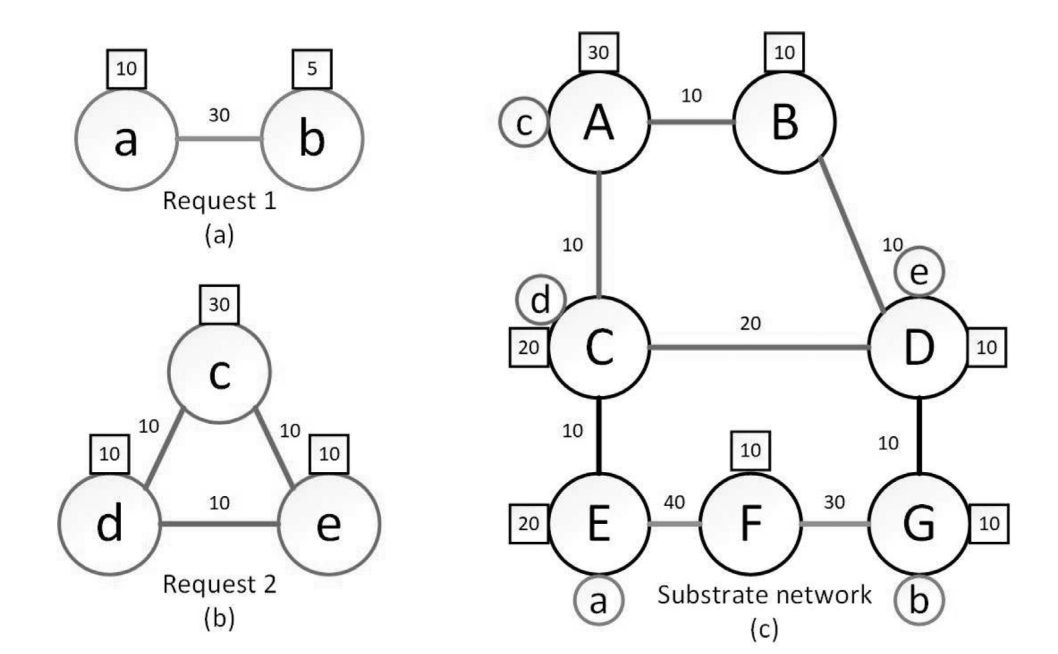
\includegraphics[width=0.7\linewidth]{../Images/Network}
		\caption{An example of virtual network embedding.}
		\label{fig:network}
	\end{figure}
\end{frame}

\begin{frame}
	\frametitle{Network modeling}
	\begin{itemize}
		\item {Substrate network: $G^S=(N^S,L^S,A_N^S,A_L^S)$}
		\item {Request: $G^V=(N^V,L^V,C_N^V,C_L^V)$}
		\item {virtual network embedding process can be formulated as$\to$ mapping $G^V$ to $G^S:G^S(N^V,L^V) \to G^S(N`,P`)\quad where N`\subset
		N^S,P`\subset P^S$}
	\end{itemize}
\begin{figure}
	\centering
	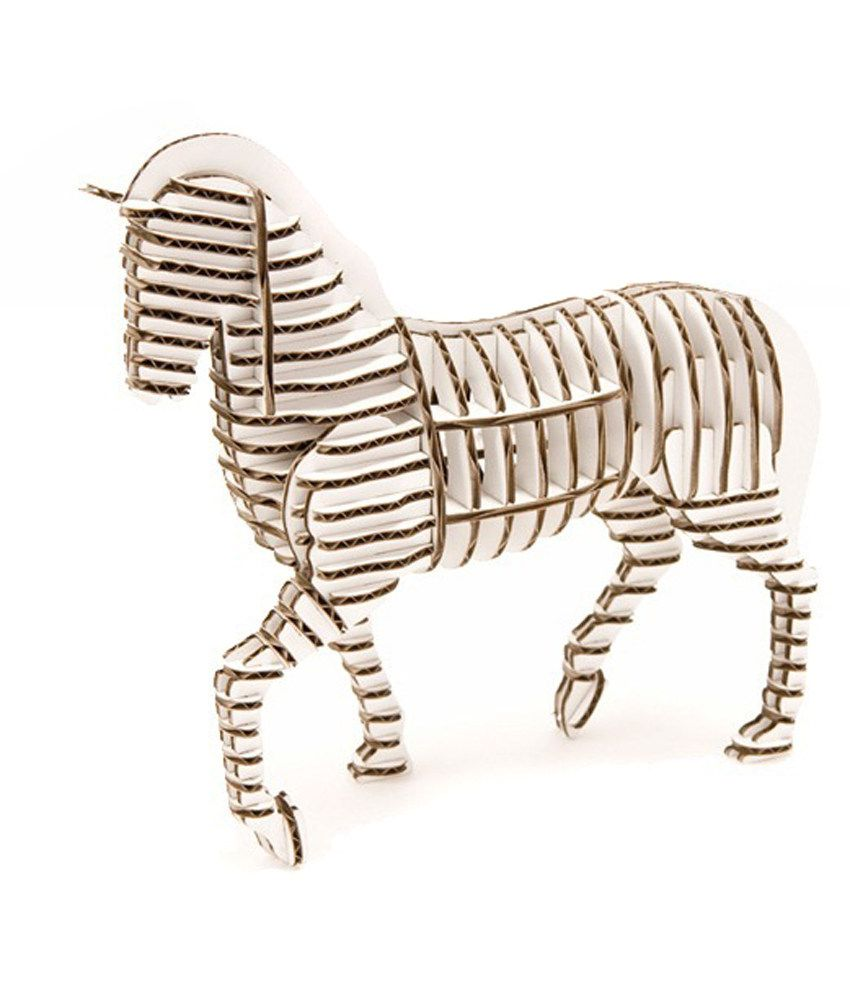
\includegraphics[width=0.4\linewidth]{../Images/modeling}
	\caption{}
	\label{fig:modeling}
\end{figure}
	
\end{frame}
\section{Policy network}
\begin{frame}
	\frametitle{Policy network}
	\begin{figure}
		\centering
		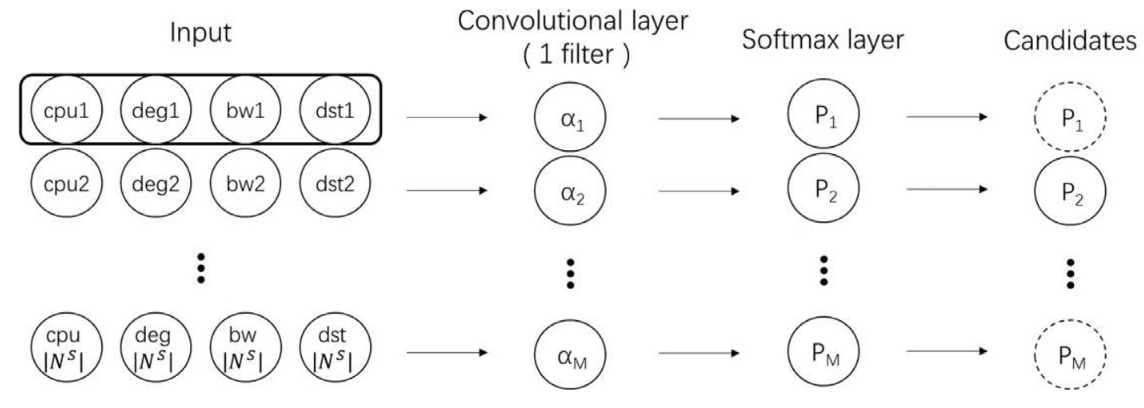
\includegraphics[width=0.9\linewidth]{../Images/policyNetwork}
		\caption{Policy network.}
		\label{fig:policynetwork}
	\end{figure}
\end{frame}
\subsection{Feature extraction}
\begin{frame}
	\frametitle{Feature extraction}
	\begin{itemize}
		\item {Computing capacity (CPU)}
		\item {Degree (DEG)\\}
		\item {Sum of bandwidth $(SUM^{(BW)})$ $ \to \quad SUM^{(BW)}(n^S)=\sum_{l^s \in L(n^S)}BW(l^S)$}
		\item {Average distance to other host nodes $AVG^{DST}$ $\to AVG^{(DST)}(n^S)=\frac{\sum_{\hat{n}^S \in \hat{N}^S}DST(n^S,\hat{n}^S)}{|\hat{N}^S|+1}$}
		\item {feature
			vector$V_K \to$\\$V_K=(CPU(n_k^S),DEG(n_k^S),SUM^{(BW)}(n_K^S),AVG^{(DST)}(n_K^S))^T$}
		\item {feature matrix $M_f$ \\
		$\to M_f=(v_1,v_2,\dots,v_{|N^S|})$}
	\end{itemize}
	
\begin{figure}
	\centering
	
\includegraphics[width=0.21\linewidth]{../Images/feature2}
	\caption{}
	\label{fig:feature2}
\end{figure}
\end{frame}
\begin{frame}
\frametitle{Feature extraction}
\begin{figure}
	\centering
	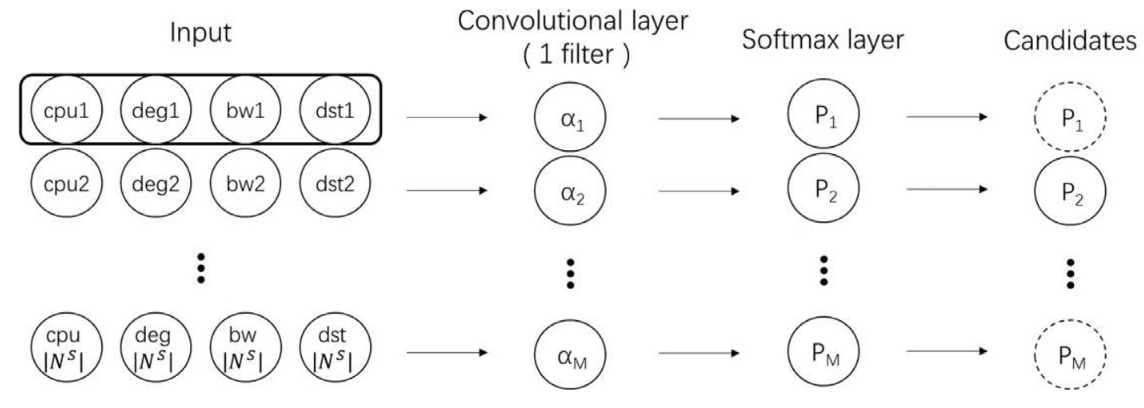
\includegraphics[width=0.9\linewidth]{../Images/policyNetwork}
	\caption{Policy network.}
	\label{fig:policynetwork}
\end{figure}
\end{frame}
\subsection{convolutional layer}
\begin{frame}
	\frametitle{convolutional layer}
	\begin{itemize}
		\item {performs a convolution operation on th input}
		\item {produces a vector representing the available
			resources of each node}
	\end{itemize}
    $\quad   h_K^c=w.v_K+b$
    
\begin{figure}
	\centering
	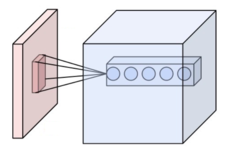
\includegraphics[width=0.3\linewidth]{../Images/Conv_layer}
	\label{fig:convlayer}
\end{figure}
\end{frame}

\begin{frame}
\frametitle{convolutional layer}
\begin{figure}
	\centering
	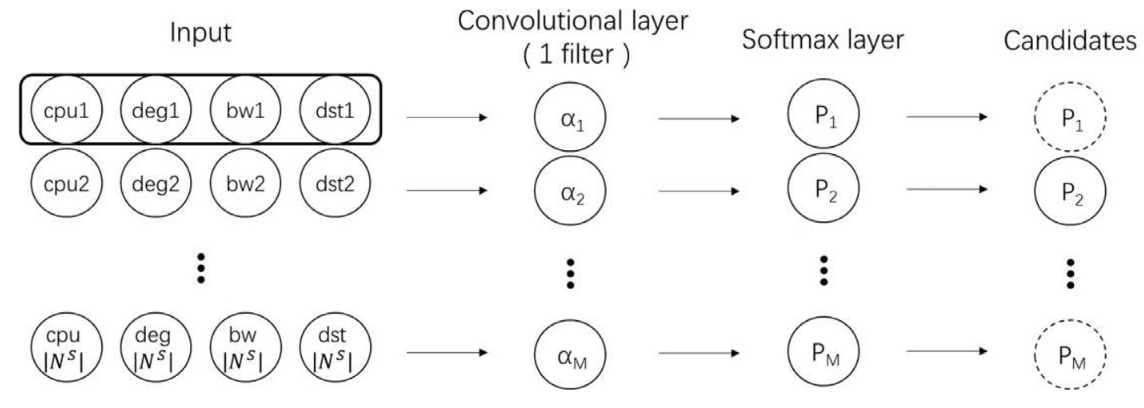
\includegraphics[width=0.9\linewidth]{../Images/policyNetwork}
	\caption{Policy network.}
	\label{fig:policynetwork}
\end{figure}
\end{frame}
\subsection{Softmax layer}
\begin{frame}
	\frametitle{Softmax layer}
	\begin{itemize}
		\item {the n-dimensional vector into real values between 0
			and 1 that add up to 1}
		\item {probability distribution over n different possible mappings}
	\end{itemize}
	$\quad p_K=\frac{e^{h_k^c}}{\sum_ie^{h_K^c}}$
	
\begin{figure}
	\centering
	
\includegraphics[width=0.3\linewidth]{../Images/softmaxLayer}
	\label{fig:softmaxlayer}
\end{figure}
\end{frame}
\subsection{Filter}
\begin{frame}
	\frametitle{Filter}
	\begin{itemize}
		\item {Some of the nodes are not able to host}
		\item{because they do not have enough computing resources}
		\item{add a filter to choose a set of candidate nodes with enough CPU
			capacities}
	\end{itemize}
\begin{figure}
	\centering
	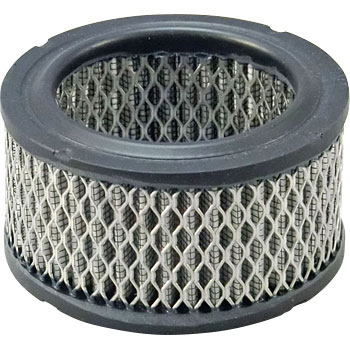
\includegraphics[width=0.3\linewidth]{../Images/filter}
	\label{fig:filter}
\end{figure}
\end{frame}
\begin{frame}
\frametitle{Softmax \& Filter}
\begin{figure}
	\centering
	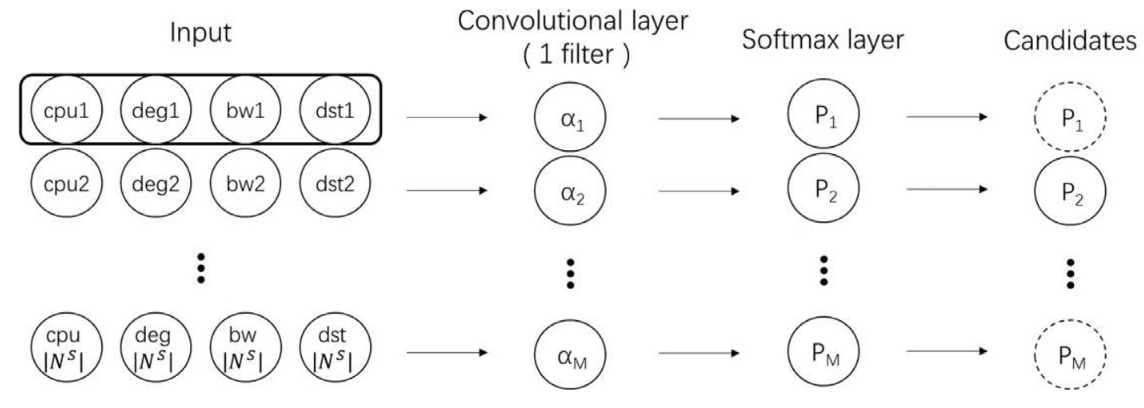
\includegraphics[width=0.9\linewidth]{../Images/policyNetwork}
	\caption{Policy network.}
	\label{fig:policynetwork}
\end{figure}
\end{frame}

\section{Training and testing}
\subsection{Training}
\begin{frame}
	\frametitle{Training}
	\begin{itemize}
		\item {randomly initialize the parameters in the policy network}
		\item{cannot simply select the node with a maximal probability as the host}
		\item {exploration \& exploitation}
		\item{ sample from the set
			of available substrate nodes according to their probability}
		\item {select a node as the
			host}
	\end{itemize}
\begin{figure}
	\centering
	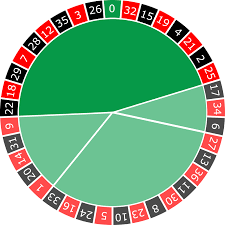
\includegraphics[width=0.3\linewidth]{../Images/roletWheel}
	\label{fig:roletwheel}
\end{figure}
\end{frame}

\begin{frame}
	\frametitle{Training}
	\begin{itemize}
		\item {repeat this process until all the virtual nodes in a virtual
			request are assigned}
		\item {proceed to link mapping}
				\item{breadth-first search to find the shortest
			paths between each pair of nodes}
		\item {If no substrate
			node is available, the mapping fails}
	\item {in reinforcement learning,  agent relies
		on reward signals to know if it is working properly}
	\end{itemize}
\begin{figure}
	\centering
	
\includegraphics[width=0.4\linewidth]{../Images/training}
	\label{fig:training}
\end{figure}
\end{frame}
\begin{frame}
\frametitle{Training}
	\begin{itemize}
		\item {If we choose the ith node $\to$ vector y filled with zeros
			except the i th position which is one}
		\item {Cross-entropy loss   $\to$   $L(y,P)=-\sum_iy_ilog(P_i)$}
		\item {use backpropagation to
			compute the gradients of parameters}
		\item {stack the gradients $g_f$}
		\item {$g=\alpha.r.g_f$}
	\end{itemize}
\begin{figure}
	\centering
	
\includegraphics[width=0.5\linewidth]{../Images/training2}
	\label{fig:training2}
\end{figure}
\end{frame}
\subsection{Testing}
\begin{frame}
\frametitle{Testing}
	\begin{itemize}
		\item {greedy strategy}
	\end{itemize}
\begin{figure}
	\centering
	
\includegraphics[width=0.4\linewidth]{../Images/Test2}
	\label{fig:test2}
\end{figure}

\end{frame}
\section{Reward}
\begin{frame}
\frametitle{Reward}	
\end{frame}
\end{document} 